
\iffalse

We provide rigorous analysis in Section~\ref{sec:definitions}. For
this motivation section we consider a confidence rated variant of Breiman's
well-known {\em Bagging}~\cite{breiman1996bagging} algorithm (for this introductory secction, we
focus on binary classification). Briefly, Bagging generates
a ensemble of $n$ decision trees. Each tree is trained on a bootstrap
re-sample from the original training set. To classify a new
example, one uses the majority vote over the trees.

\newcommand{\sign}{\mbox{sign}}
We suggest a variant of the bagging prediction rule which abstains
when the number of votes for the two labels are similar.  Let
$n_+(x),n_-(x)$ correspond to the number of trees that predict $+1,-1$
on $x$ respectively. 
The prediction rule we suggest is
\begin{eqnarray} \label{eqn:baggingWithAbstention}
  \mbox{Let }
  c(x)=\frac{|n_+(x)-n_-(x)|}{\sigma \sqrt{n}}
  \\
  P(x) =
  \begin{cases}
    -1 & \mbox{if } c(x) \leq -1 \\
    ? & \mbox{if }  -1 < c(x) < 1\\
    +1 & \mbox{if } c(x) \geq  1 
  \end{cases}
\end{eqnarray}

When $P(x) = ?$  is {\em stable} or {\em easy}, if it is small we say that
$x$ is {\em unstable} or {\em hard}.

In this paper we describe a general recipe for designing pointwise
confidence measures. We present the result of experiments using these
confidence measure and demonstrating their utility.
\fi
\section{Stability of predictions}

Consider a classification problem defined by a distribution $\cD$ over
$(x,y)$ pairs, where $x \in X$ is the input and $y \in \{1,\ldots,k\}$
is the output. A learning algorithm recieves as input a training set
$T=\langle(x_1,y_1),\ldots,(x_n,y_n) \rangle$
and outputs a classifier $c\in C$ which is a mapping from $X$ to
$Y$. The training set is drawn according to a distribution $\cT$,
which for now we assume corresponds to $n$ independent random draws
according to $\cD$, denoted $\cT = \cD^n$.

The learning algorithm projects the distribution $\cT$ into
distribution over the set of classifiers $C$ which we denote by
$\cC$.  We define global stability and pointwise stability as
follows:
\begin{itemize}
\item {\bf Global Stability} We say that
the classifer distribution $\cC$ is $(\epsilon,\delta)$-stable (globally) if with
probability $1-\delta$ over the draws of $c_1,c_2$ from $\cC$,  $\Pr{x \sim
  \cD}{c_1(x)\neq c_2(x)}\leq \epsilon$.
\item {\bf Pointwise Stability} We say that the classifer distribution
  $\cC$ is $\delta$ stable on $x$ if $\Pr{c_1,c_2 \sim \cC}{c_1(x)
    \neq c_2(x)} \leq \delta$
\end{itemize}

say that a learning algorithm has global stability with respect to
the distribution $\cD$ if two runs 

We say that the learning
algorithm is $(\epsilon,\delta)$-stable if the probability of drawing 
A deterministic learning algorithm defines a mapping from
training sets $T \in \cT$ to $c\in C$. It therefor maps the the
distribution $\cD^n$over the training sets $T$ into a distribution
over $C$.

Under the standard assumptions, the training set is drawn IID from the
distribution $\cD$. The randomness of the draw is the source of the
instability of the learning algorithm. In other words, if the learning
algorithm recieves as input the distribution $\cD$ instead of the
sample $T$ then the algorithm can be perfectly stable. In additional
to the randomness of the training set, most learning algorithm have
internal sources of instability such as the random starting point
or the order of training examples in SGD.

We therefor define 


\iffalse

\section{Pointwise confidence}

Consider a binary classification problem defined by a distribution
$\cD$ over $(x,y)$ pairs, where $x \in X$ is the input and $y \in
\{-1,+1\}$ is the output. A class of 
The most common type of stability in classification learning is
expressed in terms of uniform bounds on the difference between 


Uniform convergence theory (UCT) is the main theoretical tool for
bounding the difference between training error to test error. We call
this difference the {\em global instability} (GI).  UCT can be used to
compute upper bounds on GI.  An attractive property of UCT bounds is
that they hold {\em uniformly} for any input distribution and any
concept in the concept class. In other words, the bounds hold for the
{\em worst case} distribution, concept and learning algorithm.

Uniform bounds are attractive because they can be computed {\em
  before} the learning algorithm is executed. On
the other hand, thee bounds are inherently pessimistic. For a specific
distribution, concept and learning algorithm significantly better
bounds better bounds are possible. The idea behind ``self bounding
algorithms''~\cite{freund1998self} is that the learning algorithm,
along with the classification rule, outputs a high-probability upper
bound on the error of the same classification rule. A special case of this approach,
often called ``data-dependent complexity bounds'', has been studied by
a number of authors~\cite{}.

In this paper we refine the notion of a self bounding
algorithm to be an algorithm that outputs {\em pointwise stability
bounds} In other words, for any test point, the learning algorithm
outputs a prediction of the output, together with a bound on the
stability of the prediction. 

\section{pointwise stability}

For the sake of simplicity, we restrict our discussion to learning
$k$-class classification tasks.

A learning algorithm takes as input a training set $\cT$ and 
outputs a classifier $f$. Let $x$ be a fixed test example whose
classification is $f(x)$, our goal is to quantify the stability of
this classification.

The training set is assumed to be generated by IID draws from a fixed
unknown distribution $\cD$.  As 


We start by justifying the variant of Bagging presented in
Equation~(\ref{eqn:baggingWithAbstention}). Let $T$ be a training set
of size $m$ and let $\cD$ be the distribution over size $n$ samples
generated by bootstrap sampling from $T$. In other words, each
bootstrap sample is generated by sampling $m$ examples from $T$ with
replacement. Bagging (a.k.a. Bootstrap aggregation) consists of
generating $n$ bootstrap samples and running a fixed algorithm on them
to generate $n$ classifiers $c_1,\ldots,c_n$.

\newcommand{\te}{\tilde{e}}

Fixing any particular instance $x$, and choosing $c$ using the
bootstrap process describes above, results on a binomial distribution
over $c(x) \in \{-1,+1\}$. We denote the expected value of this distribution
by $e \doteq E\left( c(x) \right)$. The labels
$c_1(x),\ldots,c_n(x)$ are independent samples from the distribution.
Note that $e$ is a constant, not a random variable, therefor, if we
defined our prediction as a function of $e$ our prediction would be
perfectly stable. In reality we only
have the samples $c_1(x),\ldots,c_n(x)$ from which we can calculate
an estimate of $e$ namely $\te = \frac{1}{n} \sum_{i=1}^n c_i(x)$

Estimating the sign of $e$ from the estimate $\te$ is an
elementary calculation. Here we use Hoeffding bound:
\begin{equation}
  P\left( |e -\te| \geq \epsilon \right)
  \leq e^{-n \epsilon^2}
\end{equation}
\fi



\iffalse
\begin{figure}[h]
\begin{center}
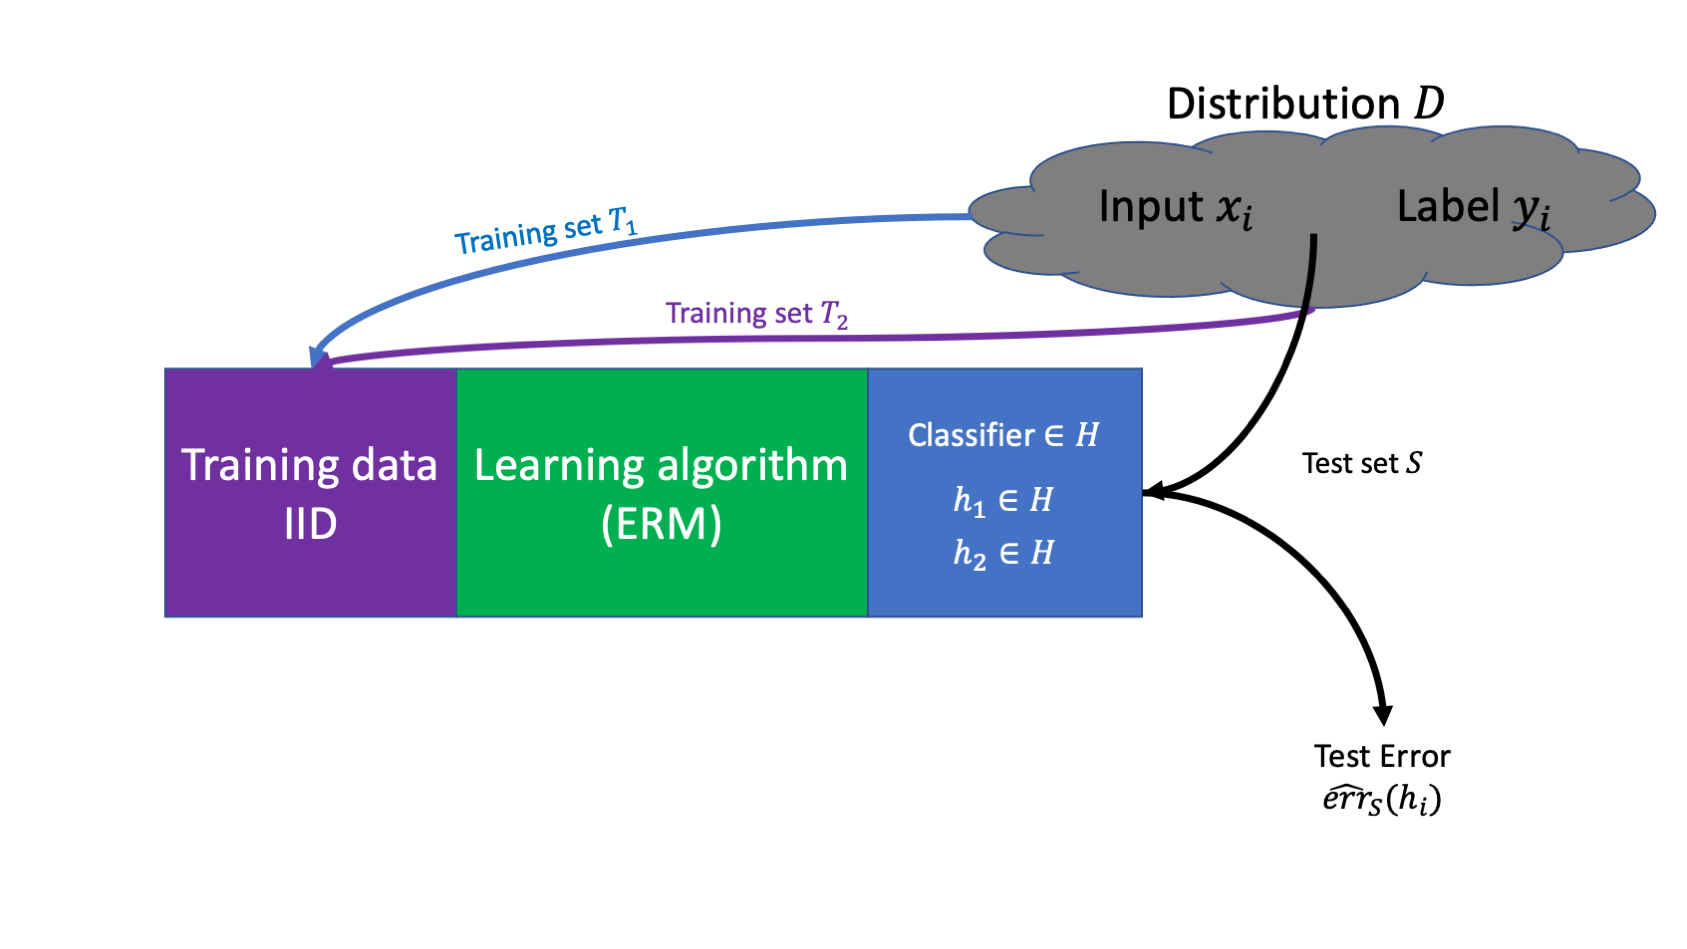
\includegraphics[width=2.75in]{PPTFigures/Uniform-Bound.png}
\end{center}
\caption{Global stability}
\label{fig:rationale}
\end{figure}

\begin{figure}[h]
\begin{center}
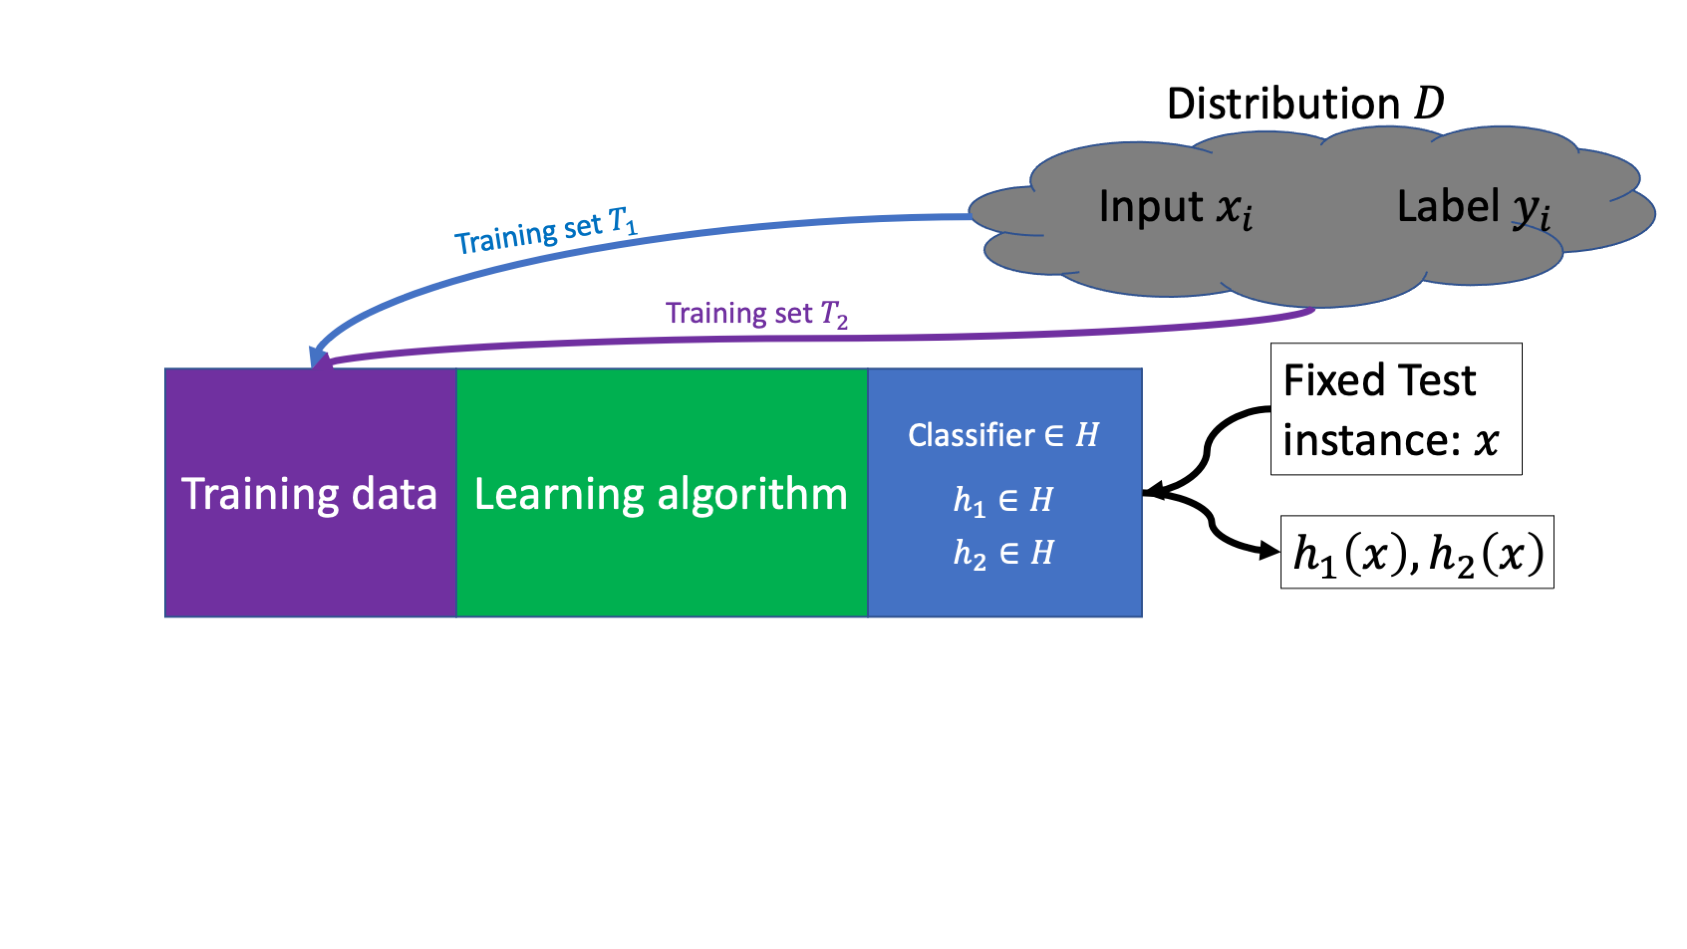
\includegraphics[width=2.75in]{PPTFigures/Pointwise.png}
\end{center}
\caption{Pointwise Stability}
\label{fig:rationale}
\end{figure}
\fi

\section{Variations}
This framework can be used in many scenarios. We list a few here:
\begin{itemize}
    \item {\bf IID} This is the classical setup where examples are drawn IID from a fixed but unknown distribution. The distribution $\cT$ is the product distribution over this fixed underlying distribution. This is the common setup for uniform convergence bounds for samples of size $n$. 
    Suppose we have an unlimited source of examples. In this case we can generate an infinite number of samples of size $n$ and compute the models uncertainty exactly.  A popular approximation for this imaginary setup is to use bootstrap: sample $n$ points with replacement from the original sample of size $n$. Bootstrap is the technique underlying Bagging~\cite{} and Random Forests~\cite{}.
    \item {\bf randomized starting point} One of the common techniques used to generate an ensemble of NN is to run the algorithm multiple times, each time with a different initial setting of the random weights.
    \item {\bf personalising} A common
\end{itemize}

\section{Boosting Distribution Margin}
\label{sec:boosting_distribution_margin}
\section{Easy and Hard Examples}
\label{sec:easy_ad_hard_examples}
\section{Algorithm}
\label{sec:algorithm}
\section{Experiments}
\label{sec:experiments}
\section{Conclusion}
\label{sec:conclusion}
% Acknowledgements should only appear in the accepted version.
\section*{Acknowledgements}

% This document was modified from the file originally made available by
% Pat Langley and Andrea Danyluk for ICML-2K. This version was created
% by Iain Murray in 2018, and modified by Alexandre Bouchard in
% 2019 and 2020. Previous contributors include Dan Roy, Lise Getoor and Tobias
% Scheffer, which was slightly modified from the 2010 version by
% Thorsten Joachims & Johannes Fuernkranz, slightly modified from the
% 2009 version by Kiri Wagstaff and Sam Roweis's 2008 version, which is
% slightly modified from Prasad Tadepalli's 2007 version which is a
% lightly changed version of the previous year's version by Andrew
% Moore, which was in turn edited from those of Kristian Kersting and
% Codrina Lauth. Alex Smola contributed to the algorithmic style files.
